\section{Preliminary results}

\label{sec:results}

Prior to 2022, seating was arranged on a first-come, first-served basis at the Palacio Nacional, which led to criticism as many journalists felt that the process was biased, favoring those aligned with the government over independent or opposition voices\citep{Tombola-Razon}. These journalists would often arrive as early as 1 a.m. to secure front-row seats. In response, the President proposed a lottery system to determine seating. By April 2022, the government formalized this change, announcing that journalists would be randomly assigned to the first three rows, with one journalist per row from each type of media—radio, television, print, etc \citep{Tombola-Financiero}. 

An important assumption in using the lottery assignment to instrument the number of critical or favorable articles written by news outlets is demonstrating that the lottery assignment actually influences which outlets get to ask questions during the press conference. If the president continues to select media outlets that are not critical of the government after the lottery—outlets that also receive more advertising revenue—two scenarios could emerge.

First, the first stage and the reduced form could become insignificant because the lottery assignment would not affect the behavior of journalists. If journalists perceive they have no real chance of participating, their seating row would not alter their approach.

Second, if the first stage is significant, it could indicate a change in journalists’ behavior. In this case, journalists might begin asking more favorable or easy questions to increase their chances of being selected. This behavioral shift would introduce endogeneity into the instrument, as the number of articles written and the advertising revenue received during that period would then become correlated with the journalists’ strategic behavior, undermining the validity of the instrument.

It is crucial to establish that the seating assignment did not alter the president's behavior and that journalists seated in the first and second rows continued to receive preferential opportunities to ask questions. Since I do not yet have complete data on attendance, seating arrangements, and question-asking patterns, I conducted the following preliminary analysis to provide some initial evidence.

\subsection{Importance of Row Seating}

To examine this, I divided the analysis into two periods: one year before the implementation of the lottery and one year after its implementation. I randomly selected 10 press conferences (five from each period) and recorded data on which journalists asked questions and where they were seated. Table \ref{tab:lottery} presents the descriptive statistics for both periods, offering insights into the changes, if any, in seating and question-asking dynamics. First thing to emphasize is that first row seating is crucial for asking questions in both periods of time. Around 70\% of the questions asked come from journalists seated in the front row. Also, this initial analysis suggests that being seated in the the third or fourth row basically decreases your chances of asking a question by a lot, which could also elicit some behavior on journalists.

\begin{table}[!htpb]
    \centering
    \caption{Descriptive Statistics of Questions Asked}
    \label{tab:lottery}
    \begin{tabular}{cccccc}
\hline \\
Time Period & Total Questions & First Row & Second Row & Third Row & Fourth Row \\
\hline\\
 Before lottery & 27 & 18 (66.67\%) & 7 (25.92\%) & 2 (7.42\%) & 0 \\
 After Lottery & 18 & 14 (77.78\%) & 2 (11.11\%) & 0 & 2 (11.11\%) \\
 Both & 45 & 32 (71.11\%) & 9 (20\%) & 2 (4.44\%) & 2 (4.44\%) \\
\hline \\[-1.8ex]  \multicolumn{6}{l} {\parbox[t]{15cm}{\small \textit{Notes:}  Descriptive statistics of the morning press conferences revised at random from the two relevant time periods. Before the lottery refers to 1 year before April 2022, and after the lottery refers to one year after. Total questions is the total number of questions asked on the respective press conference for each time period. Columns 3-6 refer to how many questions were asked from each respective row.}} \\
\end{tabular}
\end{table}

It is important to note that I am not assuming the two periods are directly comparable, as they are inherently different. For example, based on my observations of the press conferences, the dynamics in 2021 were significantly different from those in 2023. In 2021, COVID-19 safety measures, such as social distancing, face masks, and limits on the number of attendees in enclosed spaces, were in effect. These restrictions led to noticeable differences, such as a significantly smaller number of journalists present in 2021 compared to 2023, when these measures were no longer in place. This for example, could explain why there was a decrease in the total number of questions asked across periods.

Despite these changes, Table \ref{tab:lottery} highlights one aspect that remained consistent across periods: the preference given to first-row journalists when asking questions. Additionally, it is important to emphasize that my analysis will only focus on the period after the lottery was implemented. The pre-lottery period is included only for initial comparisons of select variables that may help strengthen the validity of the instrument.

\subsection{Distribution of Questions Asked}

Using the official transcripts from the press conferences, I can provide additional evidence on the exogeneity of the seating assignment and its impact on the dynamics of question-asking. Leveraging GPT-3.5 Turbo through the \href{https://platform.openai.com/docs/api-reference/introduction}{OpenAI API}, I extracted relevant information from each conference. Typically, journalists introduce themselves with phrases like, "\textit{Good morning, my name is \textbf{Name X}, from \textbf{Media Outlet Y}.}" I instructed GPT to extract both the reporter's name and their media outlet affiliation for each question asked across the relevant time period. Once this data was collected, I used \href{https://huggingface.co/hiiamsid/sentence_similarity_spanish_es}{Spanish sentence similarity embedding models} to deduplicate and cluster the names and outlets. Between April 2021 and April 2023, this process identified 556 unique journalists and 496 distinct media outlets.

From this, I constructed two datasets: one at the journalist-date level and another at the media outlet-date level. These datasets allowed me to track the total number of questions each journalist and media outlet asked across both time periods. I then examined the distributions of questions asked before and after the lottery implementation. If the lottery influenced the likelihood of non-aligned journalists asking questions or increased the variance in participating journalists/outlets, we would expect to see a less skewed distribution post-lottery, with fewer outliers dominating the questioning and more equitable participation. Figure \ref{fig:periodistas_density} illustrates the distribution of questions asked by individual journalists across the two periods.

Before the lottery, some journalists asked more than 50 questions, while a significantly smaller portion asked 10–20 questions. Post-lottery, the distribution changes noticeably. Although the distribution remains skewed—likely due to some journalists attending more frequently than others—the change suggests a shift toward greater diversity in participation. This is important because selection into attending more could introduce endogeneity into the instrument if attendance is correlated with political affinity and, consequently, with the number of favorable or critical articles written by each journalist, which might also correlate with the advertising revenue received by their outlets. To address this potential issue, as mentioned in the previous section, I will include a total attendance control variable to account for this.

\begin{figure}[!htpb]
   \centering
   \caption{}
   \label{fig:periodistas_density}
   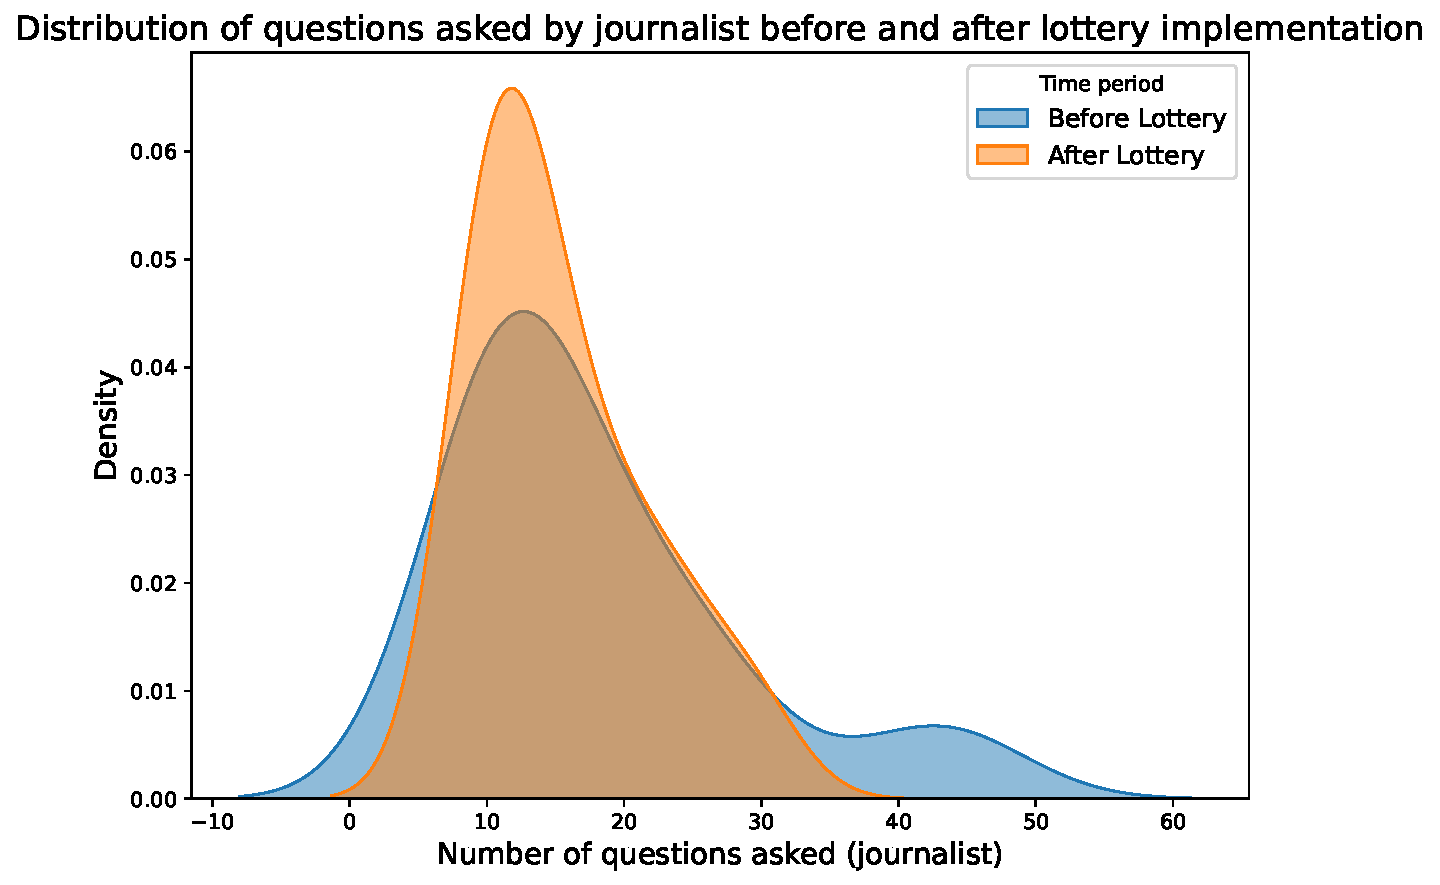
\includegraphics[width=.9\textwidth]{figures/descriptive_stats/periodistas_density.pdf}
   \caption*{ \footnotesize{\textit{Note:} This figure presents the distribution of questions asked by individual journalists across the two periods. Before lottery refers to the year before the seating arrangement lottery was implemented, on April, 2022. After the lottery refers to the year after.}}
\end{figure}

A similar pattern emerges when examining the distribution of questions asked by media outlets. Figures \ref{fig:outlet_density} and \ref{fig:outlet_density2} display the distributions for all media outlets and the top 30 outlets, respectively, during the relevant time periods. Once again, a clear shift is observed in the post-lottery period. There is a noticeable reduction in outliers—media outlets asking an exceptionally high number of questions—and an increase in the number of outlets asking a more regular amount (10–30 questions).

Additionally, when focusing on the top 30 media outlets, there is a substantial decrease in variance, and the distribution becomes more uniform. This suggests that media outlets that frequently attended the press conferences had more equal opportunities to ask questions compared to the pre-lottery period. These changes provide further evidence that the lottery system helped level the playing field, reducing the dominance of certain outlets and promoting broader participation.

\begin{figure}[!htpb]

   \centering
   \caption{}
   \label{fig:outlet_density}
   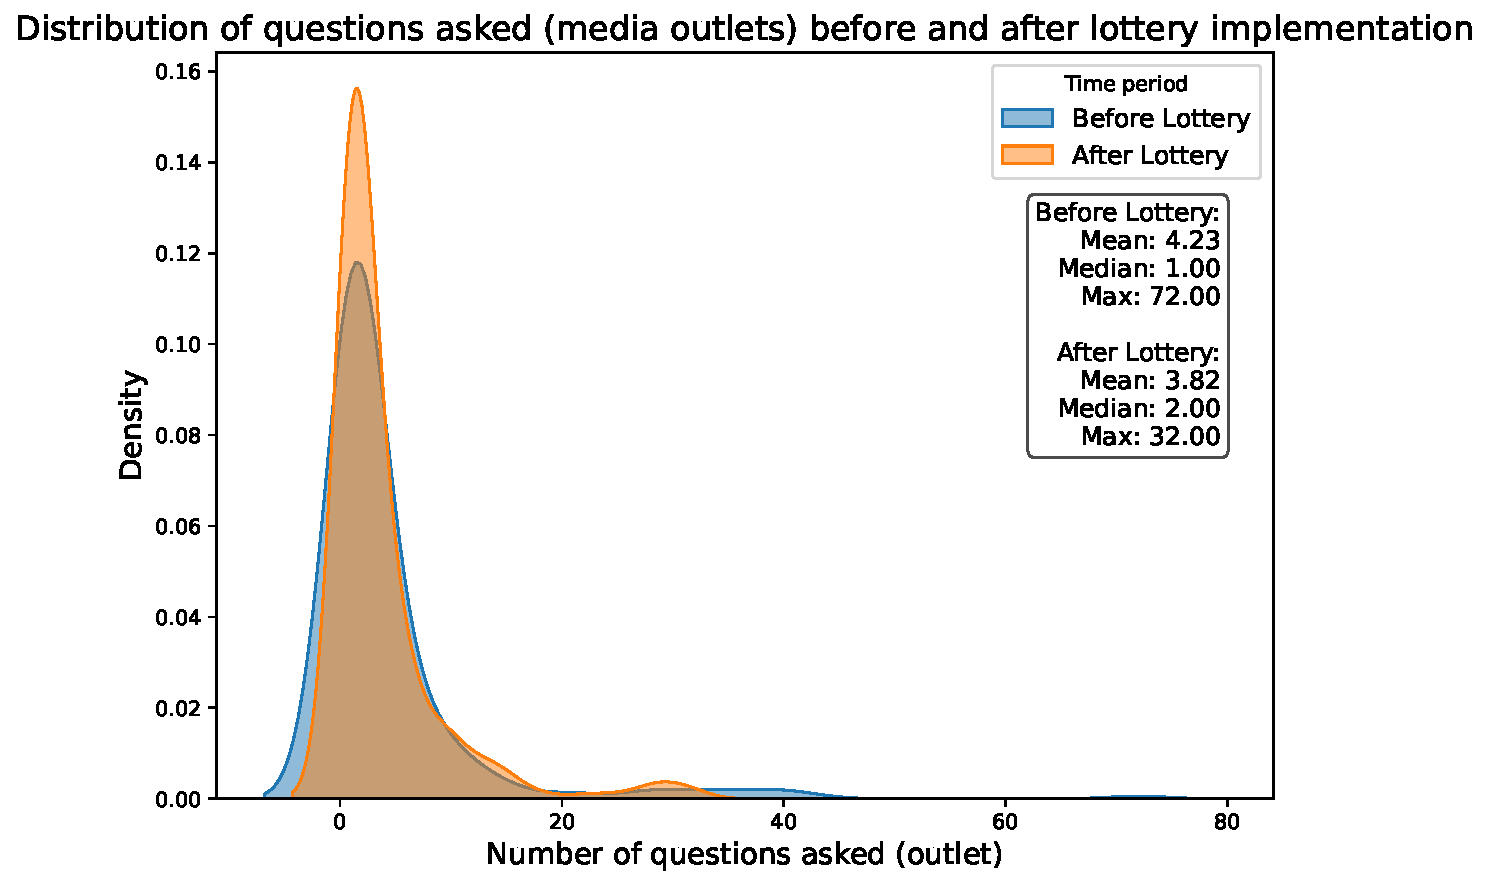
\includegraphics[width=.9\textwidth]{figures/descriptive_stats/outlet_density.pdf}
   \caption*{ \footnotesize{\textit{Note:} This figure presents the distribution of questions asked by media outlets across the two periods. Before lottery refers to the year before the seating arrangement lottery was implemented, on April, 2022. After the lottery refers to the year after.}}
\end{figure}

\begin{figure}[!htpb]
   \centering
   \caption{}
   \label{fig:outlet_density2}
   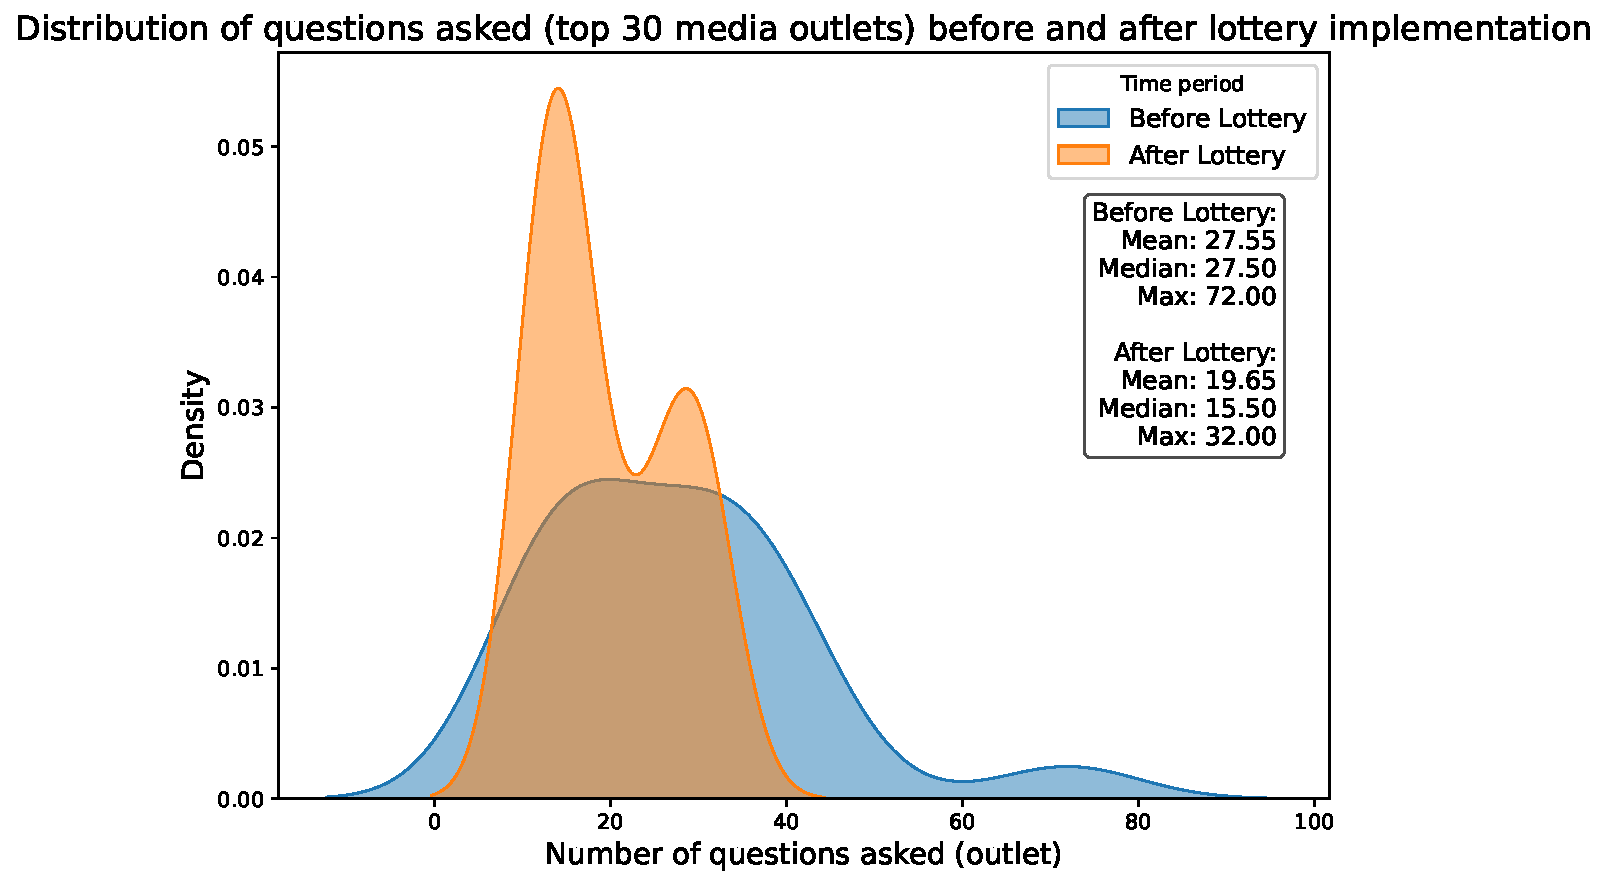
\includegraphics[width=.9\textwidth]{figures/descriptive_stats/outlet_density2.pdf}
   \caption*{ \footnotesize{\textit{Note:} This figure presents the distribution of questions asked by the top 30 media outlets that asked the most questions across the two periods. Before lottery refers to the year before the seating arrangement lottery was implemented, on April, 2022. After the lottery refers to the year after.}}
\end{figure}

Before the introduction of the lottery, most questions were asked by a small number of media outlets, likely those arriving very early each day to secure favorable seating. Importantly, these outlets could prioritize investing resources into consistently attending press conferences for several reasons. First, outlets whose content heavily relied on press conference coverage may have seen this as a way to gather official information on a wide range of topics directly from the President. Second, aligned media outlets might have benefited from asking easy or favorable questions, which could boost their viewership among the President's supporters or those aligned with the ruling party. Lastly, opposition outlets may have prioritized attending press conferences to challenge the President directly or to obtain official responses for critical reporting.

This last argument is particularly relevant when examining which outlets asked the most questions in both periods. Table \ref{tab:outlets} lists the top 10 outlets by the number of questions asked before and after the lottery was implemented. One notable observation is the consistent presence of Grupo Healy as the top question-asking outlet, represented by reporter Shaila Rosagel, who has asked the most questions overall. Interestingly, Grupo Healy is far from being an aligned media outlet, indicating their significant investment in consistently sending a reporter to the press conferences—likely arriving very early before the lottery system.

Before the lottery, several aligned outlets dominated the question-asking space. For example, Tabasco Hoy, Campeche Hoy, Quintana Roo Hoy, and Diario Basta—all owned by Grupo Cantón, whose CEO famously expressed gratitude to AMLO's administration with the phrase, "\textit{Love is repaid with love}"—were prominent in this period. These outlets serve as examples of new media organizations that likely gained viewership by producing favorable coverage of the government and heavily relying on the content generated at the morning press conferences.


\begin{table}[!htpb]
    \centering
    \caption{Top 10 Outlets that Asked the Most Questions}
    \label{tab:outlets}
    \begin{tabular}{cccc}
\hline \\
Outlet (Before) & Questions (Before) & Outlet (After) & Questions (After) \\
\hline\\
Grupo Healy & 72 &  Grupo Healy & 32 \\
 A Tiempo TV  & 42 &  La Crónica & 31 \\
 Tabasco Hoy & 40 & Frontera & 30 \\
 Campeche Hoy & 39 &  Contralínea & 29 \\
 Quintana Roo Hoy & 37 &  SDP Noticias & 28 \\
Frontera & 35 &  Proceso & 28 \\
 diario Basta & 33 &  Canal 11 & 25 \\
 La Crónica & 32 &  El Financiero & 22 \\
 Contralínea & 29 &  Noticiero en Redes. & 18 \\
 Imagen del Golfo  & 28 &  Tabasco Hoy & 16 \\
\hline
\end{tabular}
\end{table}
\end{frame}



In contrast, during the post-lottery period, the top 30 outlets saw a complete restructuring. While Grupo Healy remains at the top, the presence of opposition outlets like Proceso and El Financiero is noteworthy. These outlets are well-documented as critical of the administration. For instance, AMLO referred to Proceso as engaging in "\textit{conservative journalism, serving corrupt minorities, either directly or indirectly, consciously or unconsciously}" \citep{Attack-Proceso}. Regarding El Financiero, he once stated, "\textit{I don't want to get involved in that. Why should I give a story to your newspaper if you're against us?}" \citep{Attack-Financiero}. This shift suggests a relatively more open and equitable access to asking questions compared to the pre-lottery period.

Overall, the implementation of the lottery system appears to have reduced the dominance of aligned outlets while allowing non-aligned and critical outlets to participate more frequently. It fostered a more diverse and inclusive environment, ensuring broader representation in the press conferences.



